%\VignetteIndexEntry{geneXtendeR Vignette}
%\VignettePackage{geneXtendeR}

\documentclass[12pt]{article}

\usepackage{soul}
\usepackage{float}
\usepackage{cite}
\title{geneXtendeR}
\author{Bohdan B. Khomtchouk}

\RequirePackage{C:/Users/billy/Documents/R/win-library/3.4/BiocStyle/resources/tex/Bioconductor}

\AtBeginDocument{\bibliographystyle{C:/Users/billy/Documents/R/win-library/3.4/BiocStyle/resources/tex/unsrturl}}

\usepackage{Sweave}
\begin{document}
\Sconcordance{concordance:geneXtendeR.tex:geneXtendeR.Rnw:%
1 10 1 1 2 1 0 1 2 2 1 1 0 26 1 1 3 2 0 1 1 3 0 2 2 4 0 1 2 2 1 1 3 5 0 1 2 6 1 %
1 2 4 0 1 2 4 1 1 2 1 0 1 1 3 0 1 2 6 1 1 2 5 0 1 2 6 1 1 2 5 0 1 2 6 1 1 2 5 0 %
1 2 6 1 1 2 5 0 1 2 6 1 1 2 1 0 2 1 4 0 1 2 8 1 1 2 1 0 2 1 4 0 1 2 4 1 1 2 1 0 %
2 1 6 0 1 2 4 1 1 2 1 0 2 1 4 0 1 2 6 1 1 2 1 0 2 1 4 0 1 2 4 1 1 2 1 0 1 1 6 0 %
1 2 2 1 1 2 1 0 1 1 6 0 1 2 2 1 1 2 30 0 1 2 2 1 1 2 1 0 2 1 67 0 1 2 4 1 1 2 1 %
0 3 1 26 0 1 2 6 1 1 2 1 0 3 1 3 0 1 2 14 1 1 2 1 0 4 1 3 0 1 2 8 1 1 2 1 0 4 1 %
3 0 1 2 9 1 1 2 4 0 1 2 11 1 1 2 27 0 1 2 8 1 1 2 4 0 1 2 10 1 1 2 4 0 1 2 14 1 %
2 2 16 1 1 2 5 0 1 2 5 1 1 2 4 0 1 2 6 1 1 2 1 0 5 1 74 0 1 3 61 1}


\maketitle

\begin{figure}[H]
\centering

\includegraphics[width=50mm,scale=0.8]{figures/geneXtendeRlogo.png}
\end{figure}

\section*{Introduction}

This vignette describes \texttt{geneXtendeR} (Khomtchouk et al. 2016), an R/Bioconductor package for optimized annotation of genomic features (primarily peaks called from a ChIP-seq experiment, but any coverage island regions would work) with the nearest gene. ``Extending" refers to performing gene-feature overlaps after adding to the gene-span a user-specified region upstream of the start of the gene model and a fixed (500 bp) region downstream of the gene, resulting in assigning to a gene the features that do not physically overlap with it but are sufficiently close.  Extending is an automated iterative procedure in \texttt{geneXtendeR}, allowing the user to repeatedly align peaks to multiple gene transfer format (GTF) files to assess what global gene-spans optimize the genomewide alignment of peaks with their closest genes.  This facilitates the process of deciphering which differentially enriched peaks are dysregulating which specific genes.  This, in turn, aids experimental follow-up and validation in designing primers for a set of prospective genes during qPCR (Barbier et al. 2016).  

\subsection*{Rationale}

With an abundance of Bioconductor software currently available for peak annotation to nearby features (e.g., \texttt{ChIPpeakAnno} (Zhu et al. 2010)) as well as the existence of various command line tools (e.g., \texttt{BEDTools} \emph{closest} function (Quinlan and Hall, 2010), \texttt{HOMER} (Heinz et al. 2010)), what makes \texttt{geneXtendeR} different?  The simple answer is: \texttt{geneXtendeR} is designed for assessing the variability of peak overlap with cis-regulatory elements and proximal-promoter regions.  It is well-known that peak coordinates (peak start position, peak end position) exhibit a considerable degree of variance depending on the peak caller used (e.g., SICER (Zang et al. 2009), MACS2 (Zhang et al. 2008), etc.), both in terms of length distribution of peaks as well as the total number of peaks called, even when run at identical default parameter values (Koohy et al. 2014; Thomas et al. 2017).  Tuning algorithm-specific parameters produces even greater variance amongst peak callers, thereby complicating the issue further.  This variance becomes a factor when annotating peak lists genome-wide with their nearest genes as, depending on the peak caller, peaks can be either shifted in genomic position (towards 5' or 3' end) or be of different lengths.  As such, \texttt{geneXtendeR} represents a first step towards tailoring (or customizing) the functional annotation of a ChIP-seq peak dataset according to the details of the peak coordinates (chromosome number, peak start position, peak end position).  

The primary focus of \texttt{geneXtendeR} is to optimize the process of functional annotation of a ChIP-seq peak list whereby instead of just annotating peaks with their nearest genomic features (as statically defined by a given genome build's coordinates), \texttt{geneXtendeR} investigates how peaks dynamically align to various user-specified gene extensions (e.g., 500 bp upstream extensions, 2000 bp upstream extensions, etc. for all genes in the genome).  This shows where peaks localize across the genome with respect to their nearest gene, as well as what gene ontologies (BP, CC, and MF) are impacted at these various extension levels.  This, in turn, informs the user what gene extensions ideally capture the GO terms involved in the biology of their experiment.  For example, if a user's study is investigating the role of epigenetic enzymes in alcohol addiction and dependence, then functionally annotating a peak list using gene extensions that maximize the number of brain-related ontologies (for both BP, CC, and MF categories) makes sense.

With regards to histone modification ChIP-seq analysis, \texttt{geneXtendeR} computes optimal gene extensions tailored to the broadness of the specific epigenetic mark (e.g., H3K9me1, H3K27me3), as determined by a user-supplied ChIP-seq peak input file.  To accomplish this level of custom-tailored data analysis, \texttt{geneXtendeR} first optimally extends the boundaries of every gene in a genome by some genomic distance (in DNA base pairs) for the purpose of flexibly incorporating cis-regulatory elements, such as promoter regions, as well as downstream elements that are important to the function of the gene relative to an epigenetic histone modification ChIP-seq dataset.  This action effectively transforms genes into ``gene-spheres", a new term that we coin to emphasize the 3D-nature of heterochromatin.  A gene-sphere is composed of cis-regulatory elements (e.g., proximal promoters +/- $\approx 3$ kb from TSS), distal regulatory elements (e.g., enhancers), transcription start/end sites (TSS/TES), exons, introns, and downstream elements of a gene.  As such, \texttt{geneXtendeR} maximizes the signal-to-noise ratio of locating genes closest to and directly under peaks. By performing a computational expansion of this nature, ChIP-seq reads that would initially not map strictly to a specific gene can now be optimally mapped to the regulatory regions of the gene, thereby implicating the gene as a potential candidate, and thereby making the ChIP-seq analysis more successful. Such an approach becomes particularly important when working with epigenetic histone modifications that have inherently broad peaks with a diffuse range of signal enrichment (e.g., H3K9me1, H3K27me3). 


\section*{Quick start}

First, install the \texttt{geneXtendeR} package via:

\begin{Schunk}
\begin{Sinput}
> ## try http:// if https:// URLs are not supported
> source("https://bioconductor.org/biocLite.R")
> biocLite("geneXtendeR")
\end{Sinput}
\end{Schunk}

\begin{Schunk}
\begin{Sinput}
> library(geneXtendeR)
\end{Sinput}
\end{Schunk}

This automatically loads the \texttt{rtracklayer} R package, which contains the \texttt{readGFF()} command used to retrieve GTF files of any model organism.  As such, load in a GTF file into your R environment, e.g.:

\begin{Schunk}
\begin{Sinput}
> rat <- readGFF("ftp://ftp.ensembl.org/pub/release-84/gtf/
+                       rattus_norvegicus/Rattus_norvegicus.Rnor_6.0.84.chr.gtf.gz")
\end{Sinput}
\end{Schunk}

URLs may be obtained as direct links from: \url{http://useast.ensembl.org/info/data/ftp/index.html}.  Click on the ``GTF" link under the ``Gene sets" column for a particular species and then right-click (or command-click on Mac OS X) the name of the file containing the species name/version number and file extension \texttt{chr.gtf.gz} (e.g., Homo\_sapiens.GRCh38.84.chr.gtf.gz, Mus\_musculus.GRCm38.84.chr.gtf.gz, etc.), and copy the link address.  Then, paste the link address into the \texttt{readGFF()} as shown above.  This will create an R dataframe object containing the respective GTF file.

Next, the user must input their peak data from a peak caller (e.g., SICER, MACS2, etc.).  The peak data must contain only three tab-delimited columns (chromosome number, peak start, and peak end) and a header containing: ``chr", ``start", and ``end".  See \texttt{?samplepeaksinput} for an example.  Once the peak input data (e.g., ``somepeaksfile.txt") has been assembled properly (i.e., to contain only the three tab-delimited columns and header above), it must be properly formatted prior to the execution of downstream analyses.  

First, the user must set their working directory to point to the location of their peak data file.  Then type the following command:

\begin{Schunk}
\begin{Sinput}
> peaksInput("somepeaksfile.txt")
\end{Sinput}
\end{Schunk}

This command properly formats the user's peaks file in preparation for subsequent analyses, producing a resultant ``peaks.txt" file in the user's working directory\footnote{Similarly, users can transform their peaks file into a file of merged peaks (see \texttt{peaksMerge()}) and use the resultant ``peaks.txt" file instead for the subsequent analysis.}.

To see how the above command works using a built-in example, the \texttt{geneXtendeR} package provides a peak input dataset\footnote{This peaks dataset comes from a ChIP-seq investigation of brain tissue (prefrontal cortex) in alcohol addiction and dependence (Barbier et al. 2016), see References section for details.} called ``somepeaksfile.txt", which can be loaded into memory like this:

\begin{Schunk}
\begin{Sinput}
> fpath <- system.file("extdata", "somepeaksfile.txt", package="geneXtendeR")
> peaksInput(fpath)
\end{Sinput}
\end{Schunk}

This creates a properly formatted (i.e., properly sorted) ``peaks.txt" file in the user's working directory.

Now, we may use the R object that we created with \texttt{readGFF()} earlier to create a bar chart visualization showing the number of peaks that are sitting directly on top of genes across a series of upstream extensions (of each gene in a genome):

\begin{figure}[H]
\begin{center}
\begin{Schunk}
\begin{Sinput}
> barChart(rat, 0, 10000, 500)
\end{Sinput}
\end{Schunk}
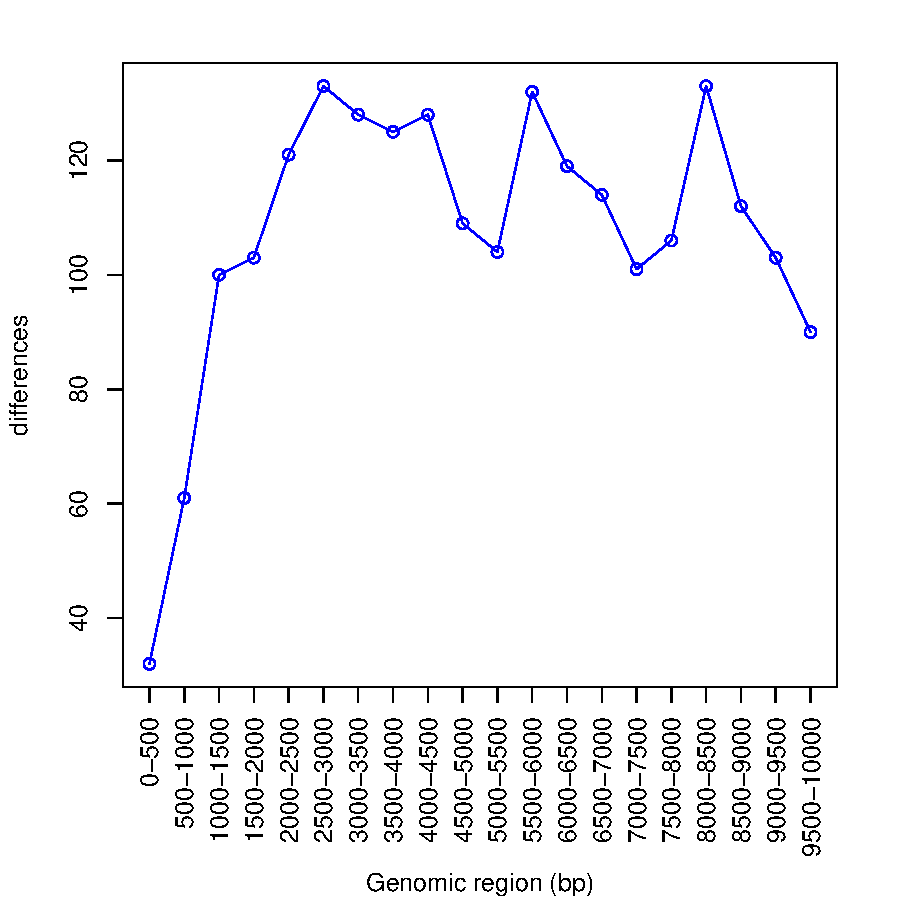
\includegraphics{geneXtendeR-007}
\end{center}
\end{figure}

This command first generates 21 individual whole-genome files: 0, 500, 1000, ..., and 10000 bp upstream extension files for the rat (\emph{Rattus norvegicus}) genome, each having an automatic 500 bp downstream extension.  In other words, each gene in the rat genome is extended upstream and downstream by some user-specified distance, thereby creating a ``gene-sphere."  As such, this bar chart command visualizes the raw count of the number of peaks that are sitting on top of genes at each individual upstream cutoff.  Clearly, the wider the gene-sphere, the more peaks-on-top-of-genes are found throughout the genome.  However, the law of diminishing returns begins to kick in at increasing upstream extension levels (see \texttt{linePlot()} for a visual representation):

\begin{figure}[H]
\begin{center}
\begin{Schunk}
\begin{Sinput}
> linePlot(rat, 0, 10000, 500)
\end{Sinput}
\end{Schunk}
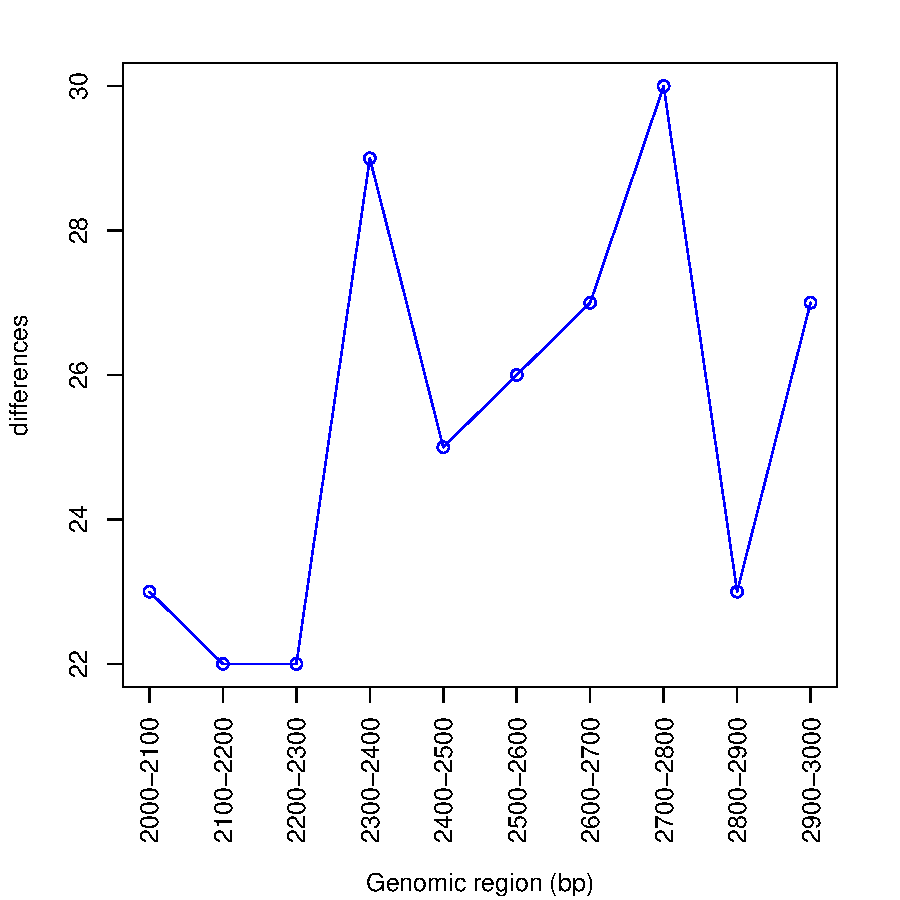
\includegraphics{geneXtendeR-008}
\end{center}
\end{figure}

In this line plot, there is a sharp rise in the number of peaks-on-top-of-genes from a 0 bp upstream extension to a 1500 bp upstream extension, and from a 2000 bp upstream extension to a 3000 bp upstream extension.  This steady rise up until 3000 bp is followed by a steady decline at subsequent extension levels followed by some noisy fluctuations.  It may be interesting to investigate what is going on in the interval from 2000 bp to 3000 bp: 

\begin{figure}[H]
\begin{center}
\begin{Schunk}
\begin{Sinput}
> linePlot(rat, 2000, 3000, 100)
\end{Sinput}
\end{Schunk}
\includegraphics{geneXtendeR-009}
\end{center}
\end{figure}

Visually, there is a relative spike in the number of peaks-on-top-of-genes at the 2400 bp upstream extension (as compared to the 2300 bp extension).  This spike then drops back down at subsequent extension levels and fluctuates in a noisy manner.  However, a cumulative line plot shows that this ``spike" is more of a visual effect than anything else, since the graph is almost perfectly linear:

\begin{figure}[H]
\begin{center}
\begin{Schunk}
\begin{Sinput}
> cumlinePlot(rat, 2000, 3000, 100)
\end{Sinput}
\end{Schunk}
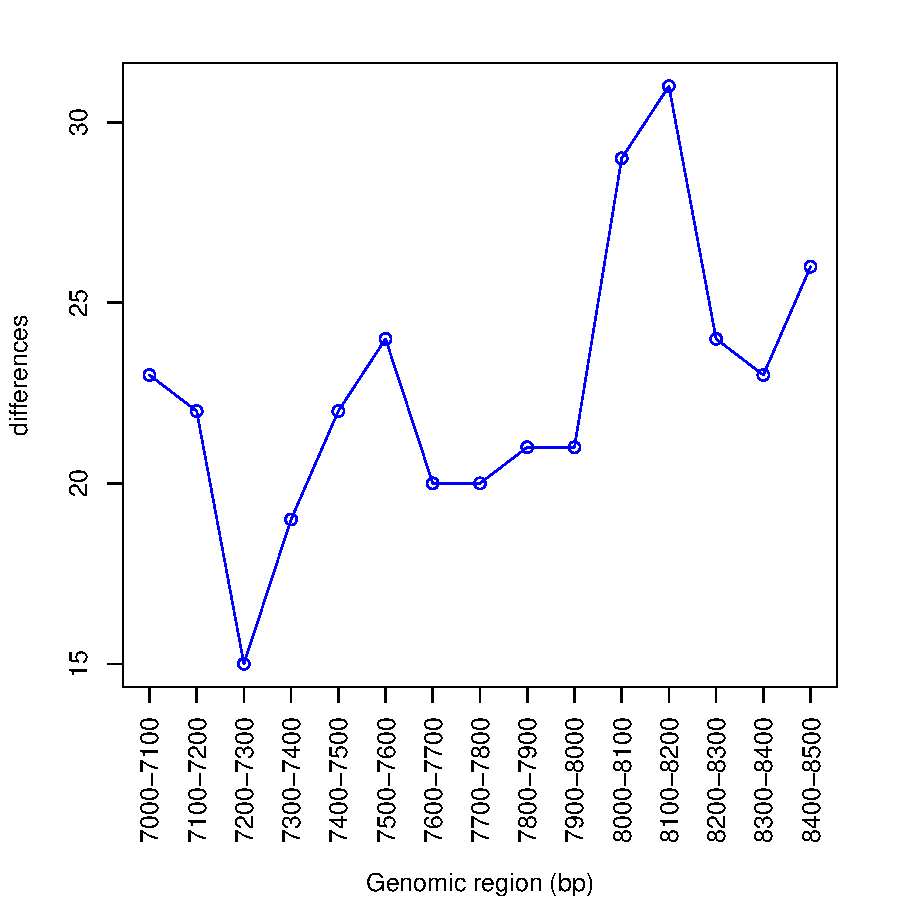
\includegraphics{geneXtendeR-010}
\end{center}
\end{figure}

Hence, one very useful function in \texttt{geneXtendeR} is called \texttt{hotspotPlot()}, which allows users to examine the ratio of statistically significant peaks\footnote{Note that statistical significance is set apriori by the user at the peak calling stage (prior to \texttt{geneXtendeR}) to give the user the freedom to choose how to filter out peak coordinates that only pass specific p-value and FDR cutoffs from a peak caller.  Peak caller output (e.g., from SICER) gives both p-value and FDR measures for each peak, thereby making it easy to extract only the peak coordinates that pass a specific set of statistical cutoff criteria.} to the total number of peaks at each genomic interval (e.g., 0-500 bp upstream of every gene in the genome, 500-1000 bp upstream of every gene in the genome, etc.). 

\begin{figure}[H]
\begin{center}
\begin{Schunk}
\begin{Sinput}
> allpeaks <- system.file("extdata", "totalpeaksfile.txt", package="geneXtendeR")
> sigpeaks <- system.file("extdata", "significantpeaksfile.txt", package="geneXtendeR")
> hotspotPlot(allpeaks, sigpeaks, rat, 0, 10000, 500)
\end{Sinput}
\end{Schunk}
\includegraphics{geneXtendeR-011}
\end{center}
\end{figure}

This line plot shows that the concentration of significant peaks in this dataset (Barbier et al. 2016) is highest between 0 and 1000 bp upstream of a gene, with over 90\% of peaks in these regions being statistically significant.  In contrast, between 1000 bp and 2500 bp, only about half of the total peaks contained in these intervals are significant.  Statistical significance then fluctuates noisly at further upstream genomic intervals, but with at least a quarter (25\%) of the total peaks in these further upstream regions being statistically significant.  As such, the take-home message is that genomic regions within the first 1000 bp upstream of their respective genes are most likely to contain significant peaks (relative to the total peak count in these regions) and are therefore hotspots, but regions beyond this also contain a fair share of statistically significant peaks.

One interesting area to investigate is the variance in the broadness of significant (or total) peaks across different genomic intervals\footnote{One can either observe the global distribution of peak lengths within specific genomic intervals (see \texttt{?peakLengthBoxplot()}), or observe the global distribution of peak lengths across all intervals (see \texttt{?allPeakLengths()}).}.  In other words, asking questions like ``are statistically significant peaks that are located very close to their nearest gene (e.g., 0-500 bp away) wider or narrower than peaks located 500-1000 bp away from their nearest gene?".  To answer this question we can do:

\begin{figure}[H]
\begin{center}
\begin{Schunk}
\begin{Sinput}
> sigpeaks <- system.file("extdata", "significantpeaksfile.txt", package="geneXtendeR")
> peaksInput(sigpeaks)
> meanPeakLengthPlot(rat, 0, 10000, 500)
\end{Sinput}
\end{Schunk}
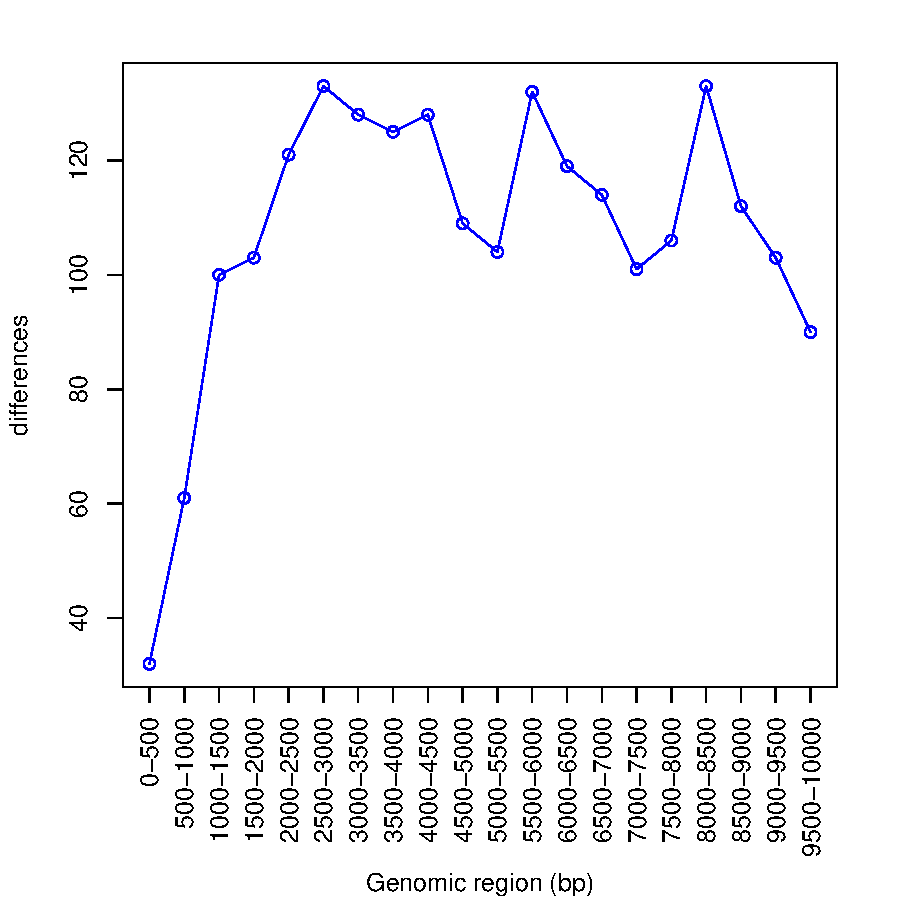
\includegraphics{geneXtendeR-012}
\end{center}
\end{figure}

This line plot displays the mean (average) length of all significant peaks found within each genomic interval.  Clearly, the ``average peak" is slightly narrower in 0-500 bp intervals than in 500-1000 bp intervals yet, overall, peak lengths tend to fluctuate more or less stochastically at various intervals.  To get the exact peak length, we can do:

\begin{Schunk}
\begin{Sinput}
> sigpeaks <- system.file("extdata", "significantpeaksfile.txt", package="geneXtendeR")
> peaksInput(sigpeaks)
> meanPeakLength(rat, 0, 500)
\end{Sinput}
\begin{Soutput}
[1] 1957.621
\end{Soutput}
\end{Schunk}

So the mean peak length in the interval 0-500 bp is approximately 1958 bp.  Although we see that there is no specific interval with peaks of extraordinary average lengths, it is still possible to see peak length outliers in certain cases (especially when looking at total peak sets):  

\begin{figure}[H]
\begin{center}
\begin{Schunk}
\begin{Sinput}
> allpeaks <- system.file("extdata", "totalpeaksfile.txt", package="geneXtendeR")
> peaksInput(allpeaks)
> meanPeakLengthPlot(rat, 0, 10000, 500)
\end{Sinput}
\end{Schunk}
\includegraphics{geneXtendeR-014}
\end{center}
\end{figure}

We see that the 4000-4500 bp and 8500-9000 bp intervals both look quite different in terms of their mean peak lengths relative to the other intervals.  To see if the mean might be influenced by a strong outlier(s), we can do:

\begin{figure}[H]
\begin{center}
\begin{Schunk}
\begin{Sinput}
> allpeaks <- system.file("extdata", "totalpeaksfile.txt", package="geneXtendeR")
> peaksInput(allpeaks)
> peak_lengths <- peakLengthBoxplot(rat, 4000, 4500)
\end{Sinput}
\end{Schunk}
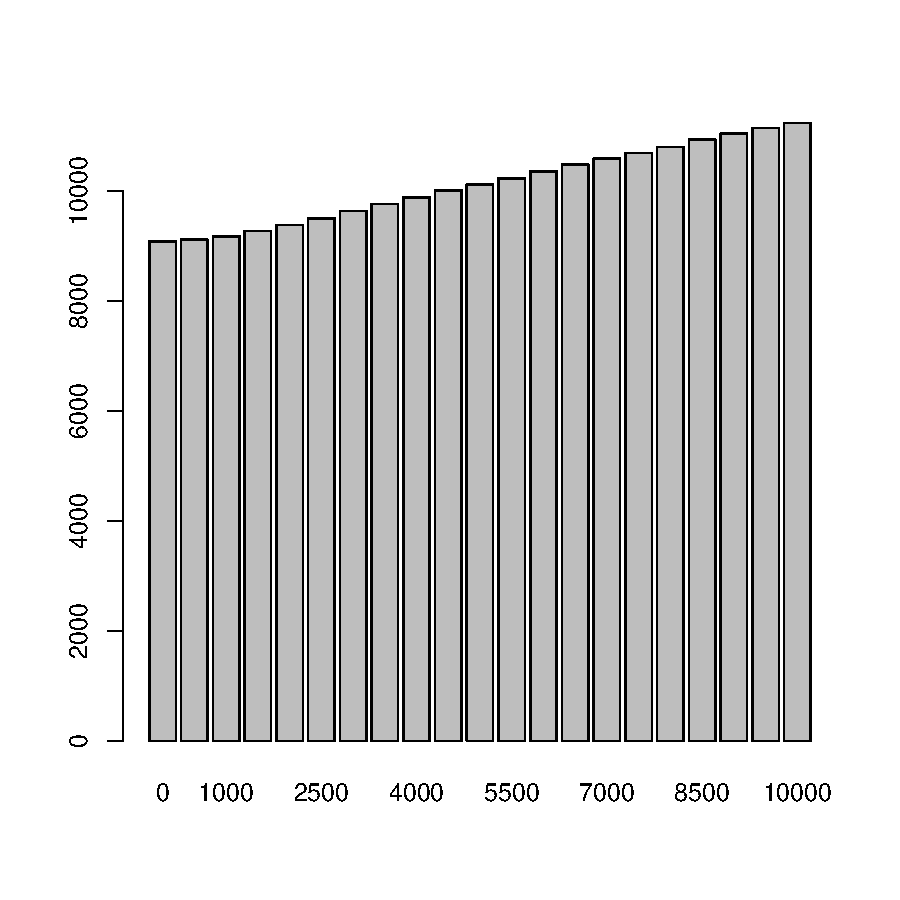
\includegraphics{geneXtendeR-015}
\end{center}
\end{figure}

This box-and-whisker plot shows a clear outlier, which is an example of a very broad peak.  We can find the exact length of this outlier peak using: 

\begin{Schunk}
\begin{Sinput}
> peak_lengths <- peakLengthBoxplot(rat, 4000, 4500)
> max(peak_lengths)
\end{Sinput}
\begin{Soutput}
[1] 114999
\end{Soutput}
\end{Schunk}

So this outlier peak measures 114999 bp in total length, therefore making it an extremely broad peak.  To see what nearest gene it resides to, we can first extract the peak's index by:

\begin{Schunk}
\begin{Sinput}
> peak_lengths <- peakLengthBoxplot(rat, 4000, 4500)
> match(114999, peak_lengths)
\end{Sinput}
\begin{Soutput}
[1] 126
\end{Soutput}
\end{Schunk}

which returns the index of where this peak length is found.  Then the following command finds all unique peaks that reside between 4000 and 4500 bp upstream of their nearest gene:

\begin{Schunk}
\begin{Sinput}
> distinct(rat, 4000, 4500)
\end{Sinput}
\begin{Soutput}
     Chromosome Peak-Start  Peak-End Gene-Chr Gene-Start  Gene-End            Gene-ID
  1:          1   19526200  19526799        1   19520708  19526671 ENSRNOG00000030796
  2:          1   61630800  61631999        1   61624941  61630954 ENSRNOG00000025949
  3:          1   71346800  71347999        1   71334629  71347133 ENSRNOG00000049014
  4:          1   98385400  98394199        1   98394160  98403468 ENSRNOG00000037331
  5:          1  101099600 101101399        1  101086377 101100094 ENSRNOG00000020583
 ---                                                                                 
124:         18   60006800  60007199       18   59985860  60007069 ENSRNOG00000017852
125:         19   45499400  45499799       19   45499420  45507827 ENSRNOG00000053551
126:         19   54877400  54992399       19   54871853  54877469 ENSRNOG00000028578
127:         20   30610800  30620799       20   30606026  30611101 ENSRNOG00000049167
128:        100   73017400  73018799      100   73018667  73024598 ENSRNOG00000027980
          Gene-Name Distance
  1: AABR07000595.1        0
  2:        Vom1r22        0
  3:   LOC100912263        0
  4:           Cd33        0
  5:          Fcgrt        0
 ---                        
124:           Nars        0
125: AABR07043877.1        0
126: AABR07044065.1        0
127: AABR07044988.1        0
128: AABR07039245.1        0
\end{Soutput}
\end{Schunk}

where we see that index \texttt{126} belongs to gene \texttt{AABR07044065.1}\footnote{This peak may not be statistically significant, but how could it be if it's so huge?  In situations like this, it may be a good idea to check what is known about the gene already: \url{http://panthertest2.usc.edu/genes/gene.do?acc=RAT\%7CEnsembl=ENSRNOG00000028578\%7CUniProtKB=A0A0G2K0W2}.  Clearly, not much is known yet.}.  Checking the arithmetic difference between column 3 and column 2 for this specific row verifies 114999, as these two columns represent the peak start position and peak end positions.  Now let's identify what the other columns represent by running the \texttt{distinct()} function again (but this time on a smaller interval to have less output printed to the screen):    

\begin{Schunk}
\begin{Sinput}
> fpath <- system.file("extdata", "somepeaksfile.txt", package="geneXtendeR")
> peaksInput(fpath)
> distinct(rat, 2300, 2400)
\end{Sinput}
\begin{Soutput}
    Chromosome Peak-Start  Peak-End Gene-Chr Gene-Start  Gene-End            Gene-ID
 1:          1   79718600  79725199        1   79725197  79728613 ENSRNOG00000026891
 2:          1  188715600 188716999        1  188688243 188715680 ENSRNOG00000016013
 3:          1  214368800 214373199        1  214373115 214386385 ENSRNOG00000018367
 4:          1  221669800 221671199        1  221671190 221694018 ENSRNOG00000027456
 5:          1  236532800 236534799        1  236529431 236532885 ENSRNOG00000022308
 6:          3   82239000  82242199        3   82096568  82239064 ENSRNOG00000008758
 7:          3   82780200  82784599        3   82762362  82780214 ENSRNOG00000042533
 8:          3  146409600 146412399        3  146376328 146409652 ENSRNOG00000006795
 9:          3  165702800 165706799        3  165678807 165702889 ENSRNOG00000042101
10:          4   84850400  84851999        4   84851986  84872257 ENSRNOG00000010205
11:          4  118157000 118157799        4  118157747 118166562 ENSRNOG00000016273
12:          4  171955800 171956999        4  171956961 171961084 ENSRNOG00000057540
13:          4  180237200 180239199        4  180231882 180237204 ENSRNOG00000048961
14:          5   36437600  36438199        5   36433358  36437694 ENSRNOG00000055329
15:          5   69038200  69039399        5   69035218  69038218 ENSRNOG00000060997
16:          5  121456000 121457199        5  121451803 121456072 ENSRNOG00000045614
17:          5  153628200 153630199        5  153568245 153628269 ENSRNOG00000018109
18:          7   14586000  14587199        7   14587120  14615369 ENSRNOG00000048450
19:          7   75225000  75225799        7   75225775  75249569 ENSRNOG00000061463
20:          8  133130600 133133199        8  133126720 133130690 ENSRNOG00000006730
21:         10    1830200   1832199       10    1832118   1841132 ENSRNOG00000040121
22:         11   80315400  80316799       11   80316777  80332099 ENSRNOG00000022160
23:         14   76654000  76654999       14   76654911  76833661 ENSRNOG00000051169
24:         14  103716400 103719199       14  103711769 103716440 ENSRNOG00000054704
25:         16     631200    642399       16     517332    631224 ENSRNOG00000061982
26:         16    9020200   9020999       16    9020987   9055164 ENSRNOG00000042628
27:         16   75363800  75364599       16   75364529  75368406 ENSRNOG00000029462
28:         20    1747000   1747399       20    1747316   1751142 ENSRNOG00000050043
29:         20   22423400  22426199       20   22420251  22423425 ENSRNOG00000057124
    Chromosome Peak-Start  Peak-End Gene-Chr Gene-Start  Gene-End            Gene-ID
         Gene-Name Distance
 1:     AC093995.1        0
 2:         Gprc5b        0
 3:         Taldo1        0
 4:       Cdc42bpg        0
 5:   LOC103691298        0
 6:        Tspan18        0
 7:          Accsl        0
 8:          Apmap        0
 9:          Zfp93        0
10:          Mturn        0
11:        Fam136a        0
12: AABR07062363.1        0
13:        Bhlhe41        0
14: AABR07047528.1        0
15:             U6        0
16:   LOC102552337        0
17:          Clic4        0
18:        Cyp4f37        0
19: AABR07057510.3        0
20:         Ccr1l1        0
21:     RGD1565158        0
22:           Rtp2        0
23:           Clnk        0
24: AABR07016558.1        0
25: AABR07024473.2        0
26:     RGD1561145        0
27:         Defal1        0
28:        Olr1735        0
29: AABR07044824.1        0
         Gene-Name Distance
\end{Soutput}
\end{Schunk}

This data table shows 29 separate entries sorted by chromosome and start position.  \texttt{V1-V3} denote the chromosome/start/end positions of the peaks, \texttt{V4-V6} denote the respective values for the genes, \texttt{V7} is the gene ID (e.g., Ensembl ID), \texttt{V8} is the gene name, and \texttt{V9} is the distance of each respective peak to its nearest gene.  It should be noted that the X chromosome is designated by the integer 100, the Y chromosome by the integer 200, and the mitochondrial chromosome by the integer 300.  This is done for sorting purposes (see \texttt{?peaksInput} for details).  In short, the \texttt{distinct()} command finds what peaks-on-top-of-genes would be missed if a 2300 bp upstream extension is used instead of a 2400 bp extension.  In other words, these 29 genes all reside between 2300-2400 bp upstream of their nearest gene.

It may be of interest to note the differential gene ontologies between these two upstream extensions:

\begin{Schunk}
\begin{Sinput}
> library(org.Rn.eg.db)
> library(GO.db)
> x <- diffGO(rat, 2300, 2400, BP, org.Rn.eg.db)
> head(x, 20)
\end{Sinput}
\begin{Soutput}
   gene$SYMBOL       GOID                                                       TERM
1       Gprc5b GO:0001934             positive regulation of protein phosphorylation
2       Gprc5b GO:0007186               G-protein coupled receptor signaling pathway
3       Gprc5b GO:0007626                                        locomotory behavior
5       Gprc5b GO:0010976       positive regulation of neuron projection development
7       Gprc5b GO:0032147                      activation of protein kinase activity
8       Gprc5b GO:0042593                                        glucose homeostasis
10      Gprc5b GO:0043123 positive regulation of I-kappaB kinase/NF-kappaB signaling
12      Gprc5b GO:0045666              positive regulation of neuron differentiation
13      Gprc5b GO:0045860             positive regulation of protein kinase activity
14      Gprc5b GO:0050729               positive regulation of inflammatory response
16      Gprc5b GO:0060907      positive regulation of macrophage cytokine production
18      Gprc5b GO:0061098    positive regulation of protein tyrosine kinase activity
20      Gprc5b GO:0090263     positive regulation of canonical Wnt signaling pathway
22      Taldo1 GO:0005975                             carbohydrate metabolic process
23      Taldo1 GO:0006002                     fructose 6-phosphate metabolic process
24      Taldo1 GO:0006098                                    pentose-phosphate shunt
25      Taldo1 GO:0009052              pentose-phosphate shunt, non-oxidative branch
26      Taldo1 GO:0019682               glyceraldehyde-3-phosphate metabolic process
27    Cdc42bpg GO:0006468                                    protein phosphorylation
29    Cdc42bpg GO:0031532                          actin cytoskeleton reorganization
\end{Soutput}
\end{Schunk}

This dataframe shows the first 20 unique gene ontology terms, their IDs, and respective gene symbols.  Clearly, gene name \emph{Gprc5b} has several BP ontologies related explicitly to the brain, while \emph{Taldo1} does not.  Considering that the ChIP-seq peaks dataset used as input into \texttt{geneXtendeR} comes from a ChIP-seq study investigating the prefrontal cortex, this suggests that a 2400 bp extension may be more suitable for this brain dataset.  However, such decisions are left entirely to the discretion and judgment of the user in deciding the relative importance of specific genes and their respective GO terms (BP, CC, or MF) to the goals of the computational analysis (as well as plans for experimental follow-up and validation).  See Discussion section for details.  

It is also critical to note that the \texttt{diffGO()} function returns ALL known gene ontologies, NOT a gene ontology enrichment analysis (more about this in Discussion section).  The goal is to provide users with knowledge regarding all possible known roles of any given gene.  For example, by knowing that a potential gene candidate has previously been linked with known brain-related ontologies, a user may be prompted to look more closely into the relevant literature behind this gene and its implications to the biological question under study (before embarking on making a decision about its potential impact and suitability as a good candidate for experimental validation).  

Furthermore, a user may plot the differential gene ontology results as an interactive network:

\begin{Schunk}
\begin{Sinput}
> library(networkD3)
> library(org.Rn.eg.db)
> library(dplyr)
> makeNetwork(rat, 2300, 2400, BP, org.Rn.eg.db)
\end{Sinput}
\end{Schunk}

\begin{figure}[H]
\centering
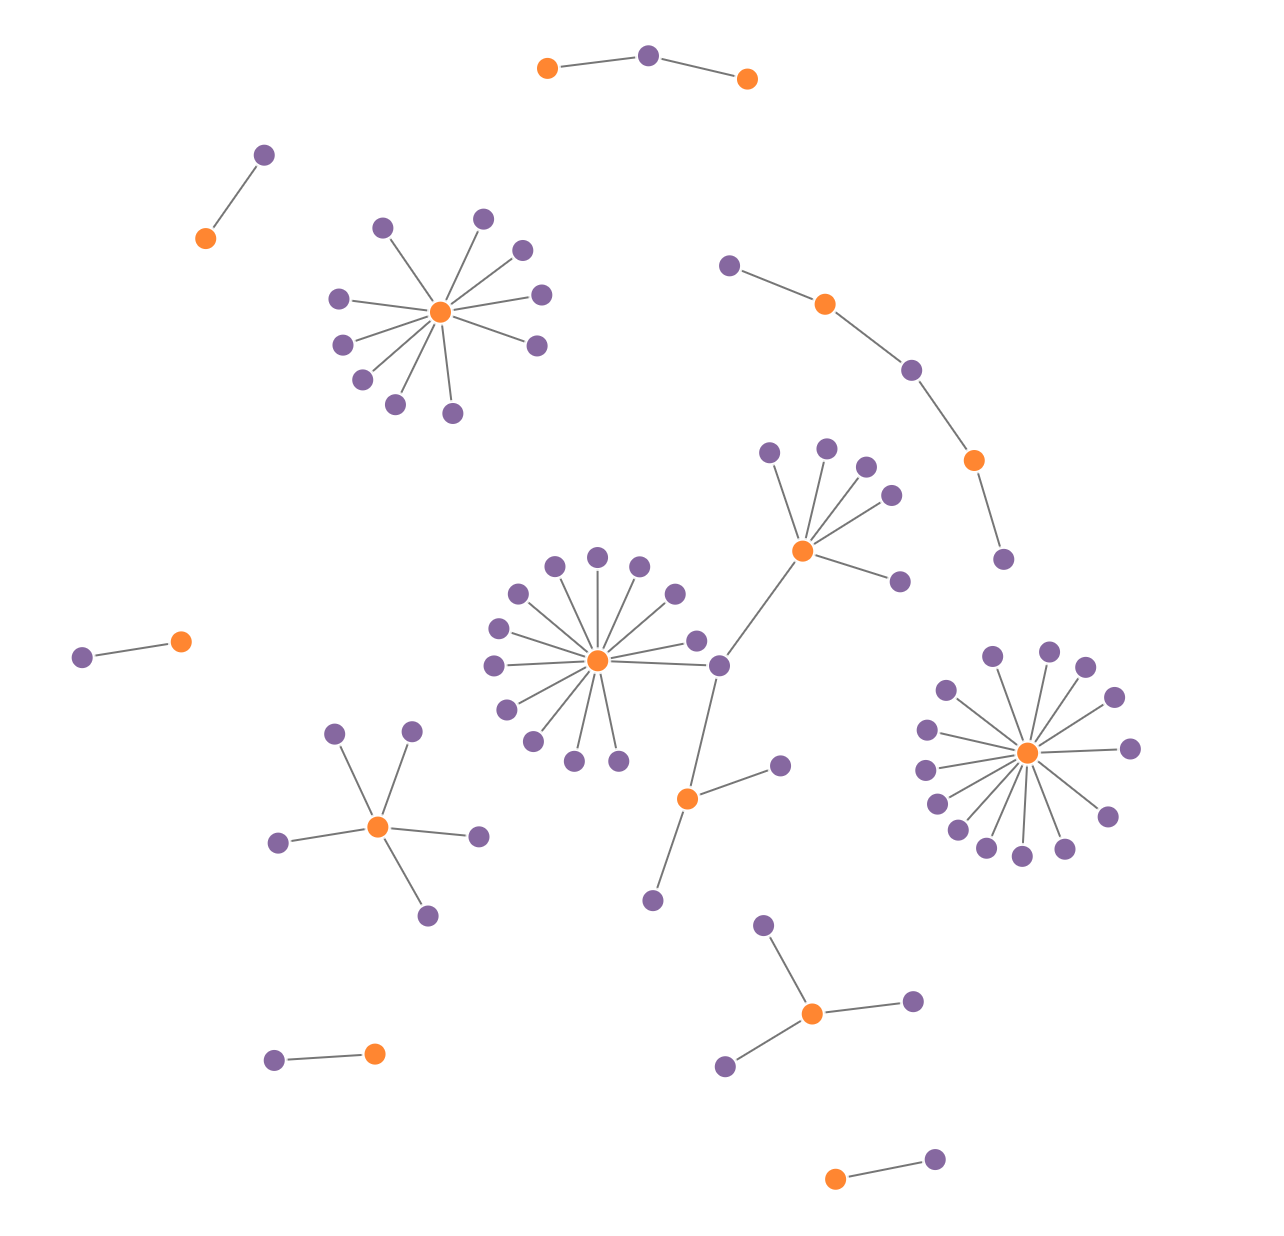
\includegraphics{figures/vignette_network_birdseye.png}
\caption{Orange color denotes gene names, purple color denotes GO terms.  A user can hover the mouse cursor over any given node to display its respective label directly within R Studio.  Likewise, users can dynamically drag and re-organize the spatial orientation of nodes, as well as zoom in and out of them for visual effect.}
\end{figure}

\begin{figure}[H]
\centering
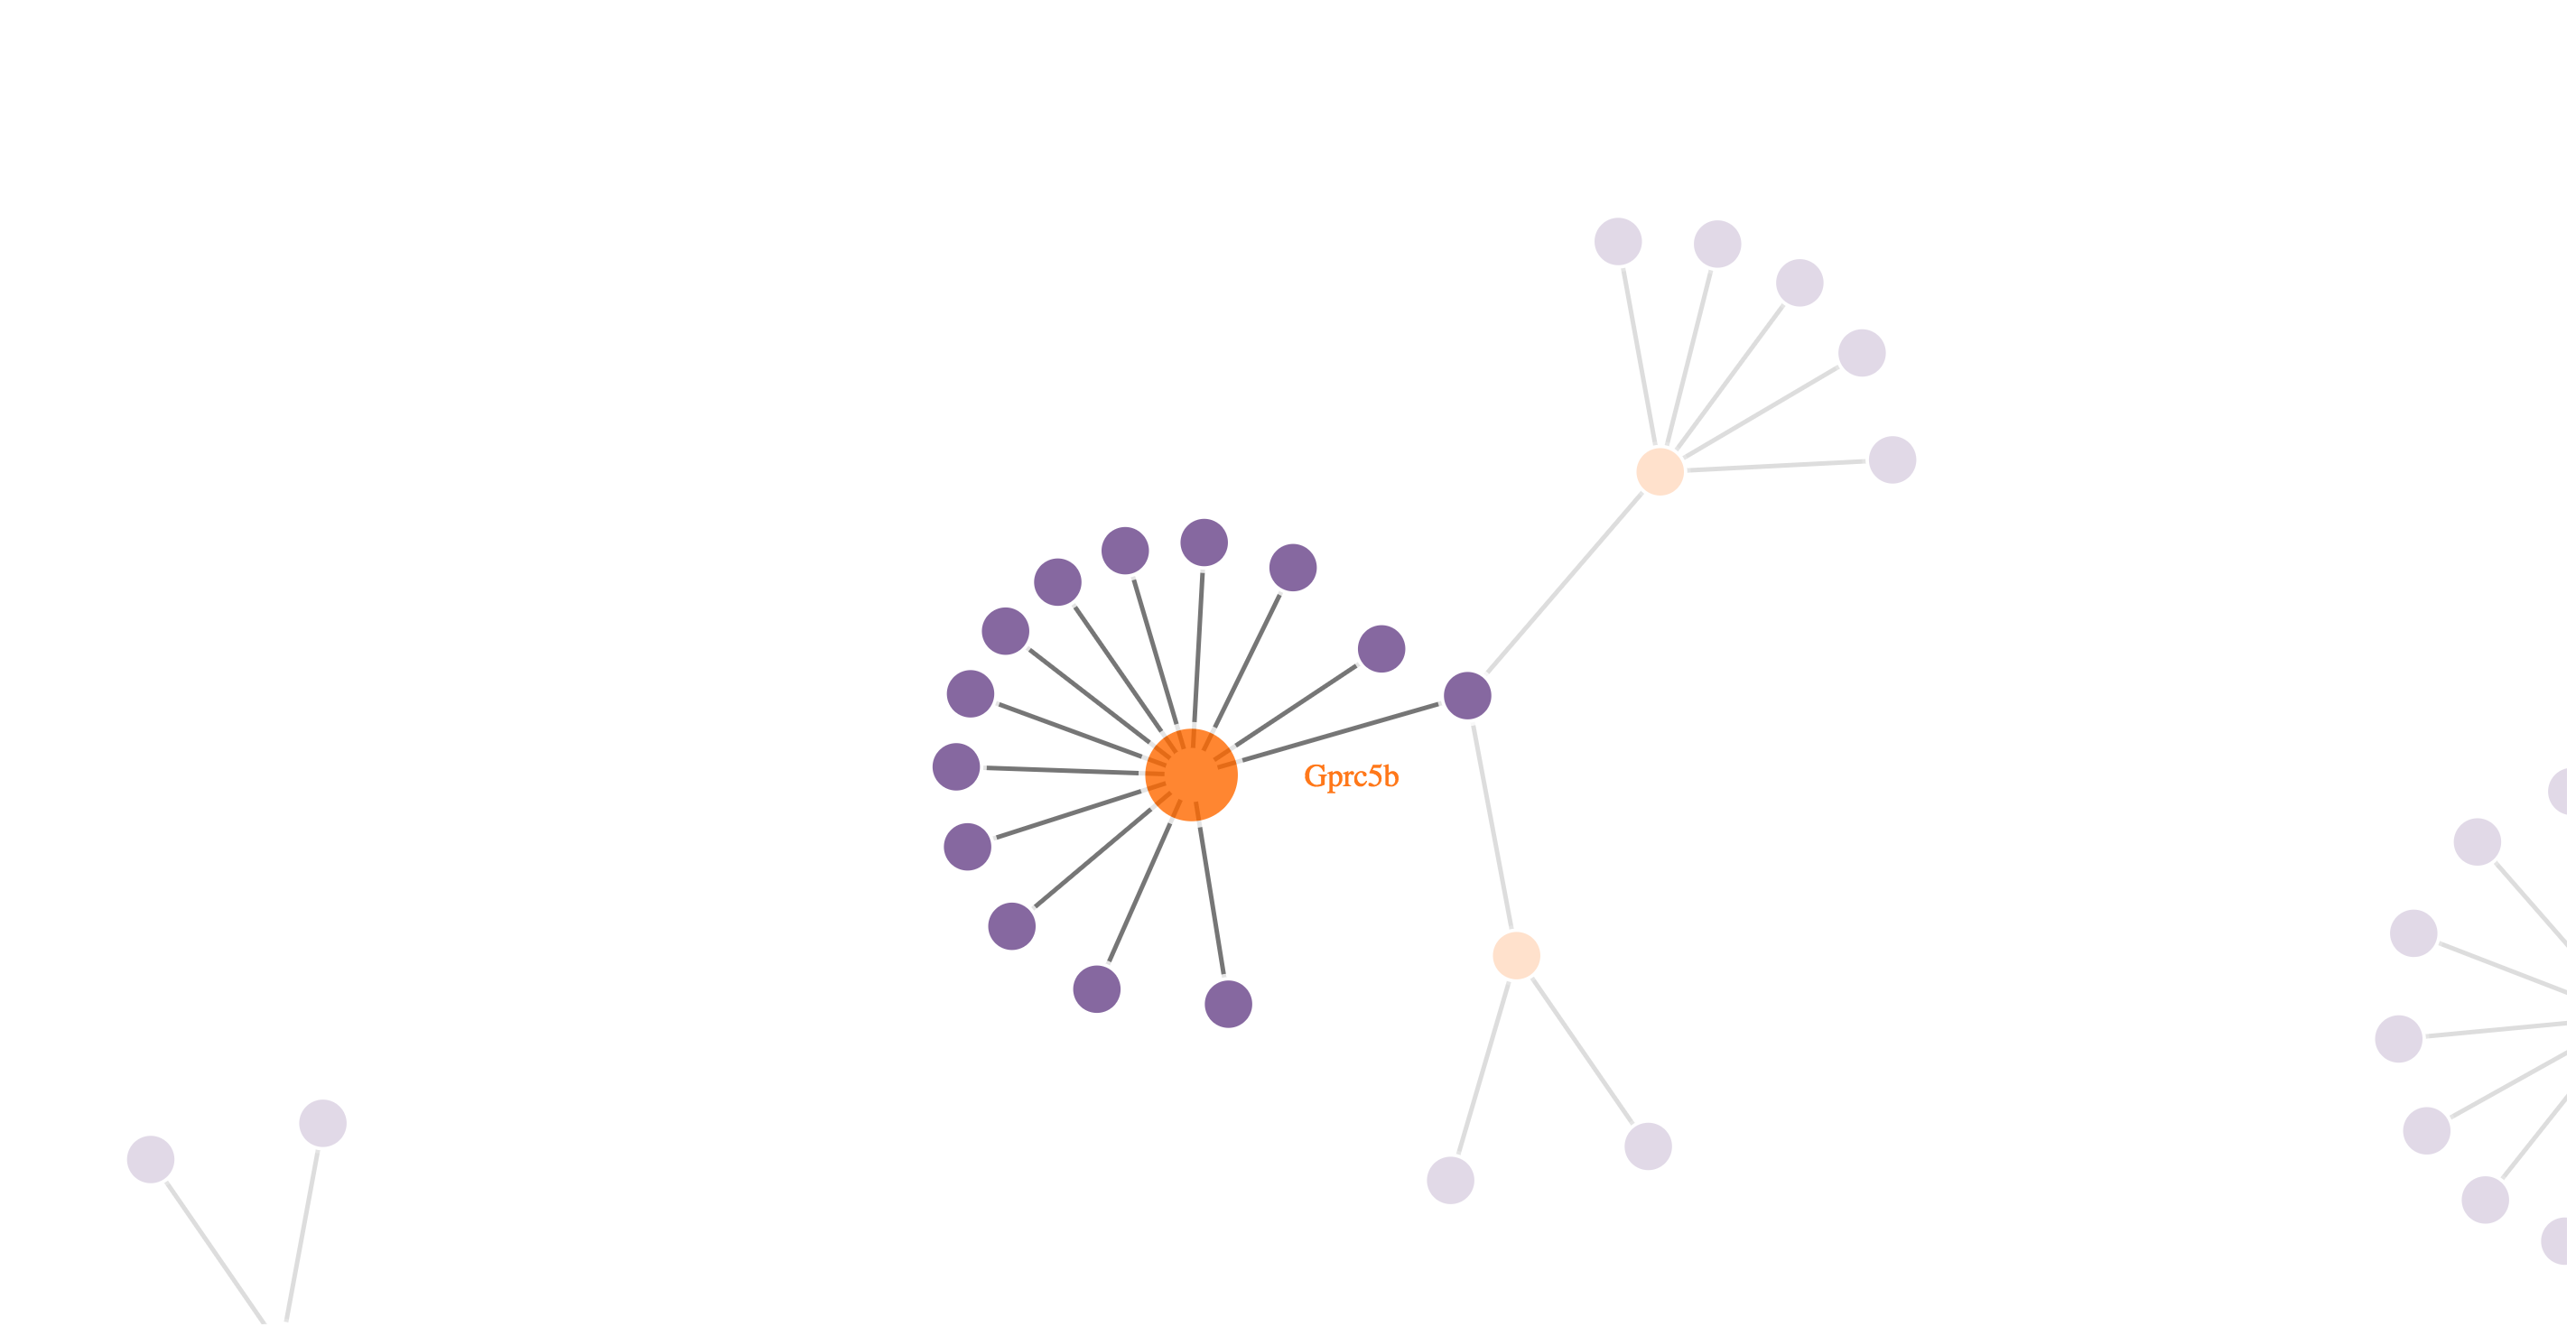
\includegraphics{figures/vignette_network_Gprc5b.png}
\caption{Orange color denotes gene names, purple color denotes GO terms.  A user can hover the mouse cursor over any given node to display its respective label directly within R Studio.  Likewise, users can dynamically drag and reorganize the spatial orientation of nodes, as well as zoom in and out of them for visual effect.}
\end{figure}

In addition, users can generate word clouds comprised from words present in their GO terms:

\begin{Schunk}
\begin{Sinput}
> library(tm)
> library(SnowballC)
> library(wordcloud)
> library(RColorBrewer)
> makeWordCloud(rat, 2300, 2400, BP, org.Rn.eg.db)
\end{Sinput}
\end{Schunk}

\begin{figure}[H]
\centering
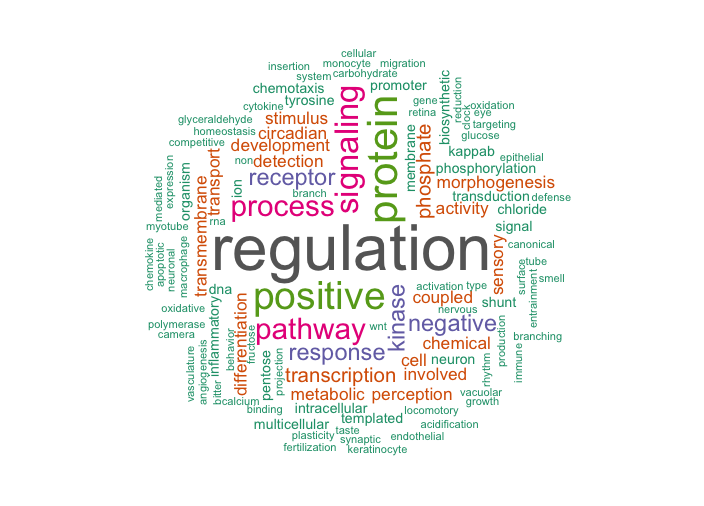
\includegraphics{figures/vignette_wordcloud.png}
\caption{Word cloud generated from words comprising gene ontology terms of category BP.  This word cloud shows the words that are used within BP gene ontology terms of peaks found to be present between 2300 and 2400 bp upstream of their nearest genes.}
\end{figure}

It may also be of interest to visually examine the most frequently used words found within GO terms:  

\begin{Schunk}
\begin{Sinput}
> library(tm)
> library(SnowballC)
> library(wordcloud)
> library(RColorBrewer)
> plotWordFreq(rat, 2300, 2400, BP, org.Rn.eg.db, 10)
\end{Sinput}
\end{Schunk}

\begin{figure}[H]
\centering
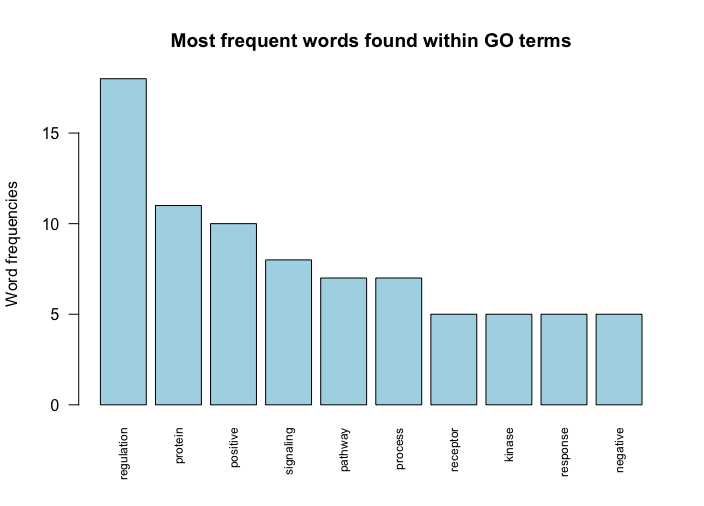
\includegraphics{figures/vignette_wordfreq.png}
\caption{This barplot shows the top 10 words used within gene ontology terms (specific to BP) of peaks found to be present between 2300 and 2400 bp upstream of their nearest genes.}
\end{figure}


Once the user has chosen the specific upstream extension to be used, the peak file is ready to be fully annotated:

\begin{Schunk}
\begin{Sinput}
> annotate(rat, 2400)
\end{Sinput}
\end{Schunk}

\begin{figure}[H]
\centering
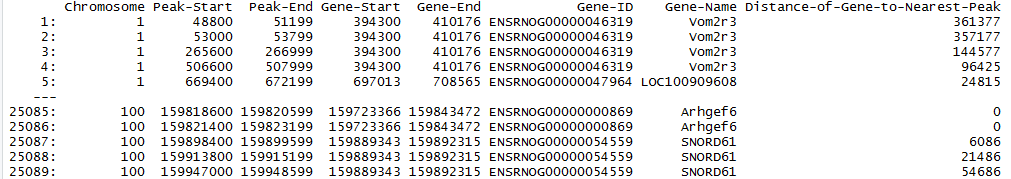
\includegraphics{figures/vignette_annotate_2400.PNG}
\caption{This output shows an example of how the data is output from the annotation function.}
\end{figure}

which generates a fully annotated peaks outfile (in the user's working directory) containing various genomic features and labeled headers.

If a user is looking for a more gene-centric approach to an\-notation, they may use either the \texttt{gene\_lookup()}
or \texttt{gene\_annotate()} functions. The \texttt{gene\_annotate()} function builds off of the \texttt{annotate()} function, but reorganizes the information based on relevant gene information.

\begin{Schunk}
\begin{Sinput}
> head(gene_annotate(rat, 2400))
\end{Sinput}
\begin{Soutput}
  Chromosome Gene-Start  Gene-End            Gene-ID Gene-Name
1         12   14448510  15101186 ENSRNOG00000001103      Sdk1
2          5  168141047 168736696 ENSRNOG00000018602    Camta1
3          8  127268889 127573488 ENSRNOG00000043167     Itga9
4         13  106749225 107427829 ENSRNOG00000003738     Ush2a
5         10   18557628  18944940 ENSRNOG00000005365    Kcnip1
6         12   51385263  51705130 ENSRNOG00000032590     Ttc28
  Number-of-Peaks-Associated-with-Gene Mean-Distance-of-Gene-to-Nearest-Peaks       sd
1                                   36                               6290.222 19899.71
2                                   21                                  0.000     0.00
3                                   20                                  0.000     0.00
4                                   20                                  0.000     0.00
5                                   19                                  0.000     0.00
6                                   19                                  0.000     0.00
  Peaks-on-Gene-Body
1                 32
2                 21
3                 20
4                 20
5                 19
6                 19
\end{Soutput}
\end{Schunk}

\begin{figure}[H]
\centering
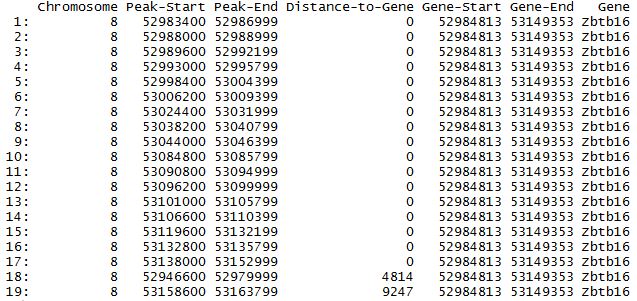
\includegraphics{figures/vignette_gene_lookup_zbtb16_19.png}
\caption{This output shows all the peaks nearest to "Zbtb16" and their respective distances. Even though only 17 of the peaks reside on the extended gene-body, the additional two peaks are close enough to consider being included in analysis.}
\end{figure}

Information such as Peaks-on-Gene-Body, number of peaks associated with a single gene, and other information are included in this table. \hl{Ideally, a user would be looking for genes that have a high number of \texttt{Peaks-on-Gene-Body} to follow-up on for gene research. Genes that have peaks that reside close to the chosen gene-body (low mean) and that are clustered (low standard deviation) may also be good targets for follow-up analysis.} The \texttt{gene\_lookup()} function looks up all genes' (or gene IDs') peaks surrounding those genes across all chromosomes and reports these peaks. \hl{This method is extremely useful when paired with \texttt{gene\_annotate()} to check genes that may be used in a follow-up.}

\begin{Schunk}
\begin{Sinput}
> gene_lookup(rat, c("zbtb16"), n = 19, extension = 2400)
\end{Sinput}
\end{Schunk}

\begin{figure}[H]
\centering
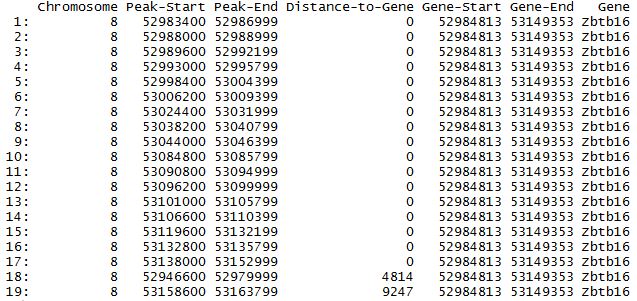
\includegraphics{figures/vignette_gene_lookup_zbtb16_19.png}
\caption{This output shows all the peaks nearest to "Zbtb16" and their respective distances. Even though only 17 of the peaks reside on the extended gene-body, the additional two peaks are close enough to consider being included in analysis.}
\end{figure}

\hl{In \texttt{gene\_lookup(organism, gene\_name, n, extension)}, n represents the number of nearest peaks to a given gene, listed separately for each chromosome. In the case of "zbtb16," there are 19 nearest peaks to the gene and this displays their location as well as their distance from the gene. This function is motivated by the need of biologists to accurately design primers for specific genomic loci in order to experimentally validate the existence (realness) of a peak.}

For a much more in-depth analysis, a function that combines both \texttt{gene\_lookup()} and \texttt{gene\_annotate()} has been provided as \texttt{annotate\_n()}. Instead of simply annotating a peak to a single, closest gene, this function annotates each peak to the closest, the second-closest, ..., to the nth-closest genes to provide the user an expanded picture of the peaks layout for further analysis. Called, this function looks like:

\begin{Schunk}
\begin{Sinput}
> annotate_n(rat, 3500, n=3)
\end{Sinput}
\end{Schunk}

\begin{figure}[H]
\centering
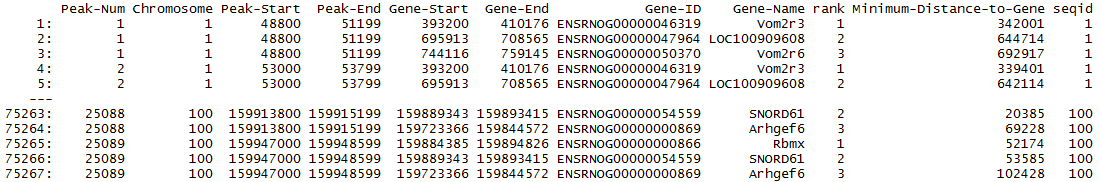
\includegraphics{figures/vignette_annotate_3500_3.png}
\caption{This output shows how the information is organized and the scale of the information provided.}
\end{figure}

\hl{This function is the most versatile of the annotation functions provided and is extremely useful for providing peak-to-gene evidence and follow-up information. When moving away from the traditional "first closest gene" to a peak, this method opens up many more possiblibilities as to which peaks influence which genes. It increases the scope of the individual peaks to reduce the chance a peak that influences any particular gene is missed or misattributed to the wrong gene.}

\section*{Discussion}

Even though \texttt{geneXtendeR} is designed to compute (and analyze/display) optimal gene extensions tailored to the characteristics of a specific peak input file, \texttt{geneXtendeR} will not explicitly impose on the user the optimal extension to select, since this information is highly study-dependent and, as such, is ultimately reserved to the user's discretion.  For example, a user may choose a conservatively lower upstream extension (e.g., for studies investigating narrow peaks such as H3K4me3 or H3K9ac that exhibit a compact and localized enrichment pattern, where high upstream extensions may begin to lose biological relevance).  An example of such a user-driven decision would be the selection of a 1500 bp upstream extension instead of a 3500 bp extension in situations like this:

\begin{figure}[H]
\begin{center}
\includegraphics{geneXtendeR-028}
\end{center}
\end{figure}

This line plot is derived from the input peak dataset used from the H3K9me1 study examined earlier (Barbier et al. 2016).  If the study had examined a narrower chromatin mark (e.g., H3K4me3) then the decision process for choosing an optimal extension may have been different.  

In certain cases, additional extensions are unlikely to add significant value to the annotation of the peak file.  Taking the example of the 0-10000 bp line plot, an upstream extension beyond 3500 bp globally across every gene in a genome would most likely not accurately reflect the biology of the peak input file (since such large global upstream extensions are likely to reach considerably beyond known proximal promoter elements, especially for relatively narrow histone marks or transcription factors).  Such assumptions may be validated directly by the user by investigating the p-value and FDR of specific peaks using a combination of \texttt{HT-seq} (to count the reads) and \texttt{edgeR}/\texttt{DESeq2} (to assess statistical significance).  As such, \texttt{geneXtendeR} is designed to be used as part of a biological workflow involving subsequent statistical analysis:

\begin{figure}[H]
\centering
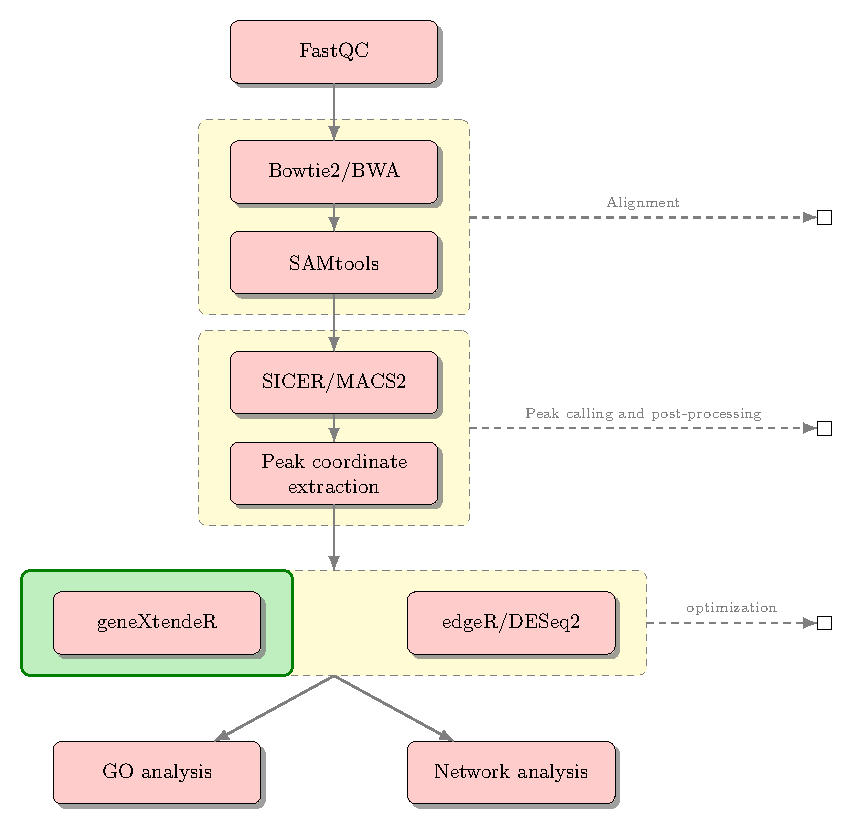
\includegraphics{figures/workflow.pdf}
\caption{Sample biological workflow using \texttt{geneXtendeR} in combination with existing statistical software to analyze peak significance.  Subsequent gene ontology enrichment or network analysis may be conducted on genes associated with statistically significant peaks.}
\end{figure}

It is entirely possible (and probable) for significant peaks to be present at relatively high upstream extension levels (i.e., large gene-spheres), albeit these significant peaks may be associated with biology not directly relevant to the study at-hand, due mainly to the sheer magnitude of the distance of the peak from traditional gene boundaries (where traditional gene boundaries may be loosely defined as +/- $\approx 3$ kb from TSS and +/- $\approx 0.5$kb from TES).  Consequently, it is likely for peaks-on-top-of-genes to exhibit higher levels of noise at higher upstream extension levels.  Nevertheless, this does not mean that potential enhancer activity should be discounted.  For instance, it is not uncommon to see a steady rise or even a surge in the number of peaks-on-top-of-genes at higher upstream extension levels:

\begin{figure}[H]
\begin{center}
\begin{Schunk}
\begin{Sinput}
> linePlot(rat, 7000, 8500, 100)
\end{Sinput}
\end{Schunk}
\includegraphics{geneXtendeR-029}
\end{center}
\end{figure}

This line plot shows that there are over 30 peaks in this dataset (across the rat genome) that reside between 8100 and 8200 bp upstream of their nearest gene.  In far-out cases like this, it is particularly recommended to examine the statistical significance of peaks to get a sense for the possibility of potential enhancer activity/regulation.  Of course, such computational findings would require experimental follow-up and/or database mining for known motifs.  Assessment of such statistical significance values is beyond the scope of \texttt{geneXtendeR}, in order to allow the user freedom to choose the most appropriate statistical package/technique for their analysis.  As before, first use the \texttt{distinct()} function to create a table of unique genes located under peaks between the two upstream extension levels:

%<<fig.width=6.2, fig.height=5>>=
\begin{Schunk}
\begin{Sinput}
> distinct(rat, 8100, 8200)
\end{Sinput}
\end{Schunk}

Then, assess the statistical significance of these peaks using a combination of \texttt{HT-seq} (Anders et al. 2015) and \texttt{edgeR} (Robinson et al. 2010), or \texttt{HT-seq} and \texttt{DESeq2} (Love et al. 2014), or some other appropriate combination of existing software tools.  Genes associated with the resultant statistically significant peaks may then be further assessed with gene ontology enrichment analysis to help answer a variety of interesting research questions.  It should once again be noted that the \texttt{diffGO()} function does NOT perform gene ontology enrichment analysis.  Instead, it returns all known gene ontologies for each gene.  The purpose and utility of this is described in the previous section.

Moreover, DNA sequences under peaks may be checked for the presence of known regulatory motifs (e.g., using \texttt{TRANSFAC} (Matys et al. 2006) or \texttt{MEME}/\texttt{JASPAR} (Sandelin et al. 2004, Bailey et al. 2009)), or for the presence of biological repeats (e.g., using \texttt{RepeatMasker} (Smit et al. 2015)). Pending a prospective GO enrichment and network analysis, functional validation may be followed up in the lab to test any potential regulatory sites or prospective enhancer elements, thereby bringing the computational analysis pipeline back to the bench.

In addition to the computational workflows discussed above, \texttt{geneXtendeR}'s wide array of functions makes it possible to conduct some rather interesting and creative combinations of genomic analysis.  Let's say, for example, that a user wants to explore all known ontological differences across specific disparate sectors of the genome (e.g., 0-500 bp vs. 2000-3000 bp, but removing 501-1999 bp from consideration).  In other words, look at all peaks (across the entire genome) that reside between 0-500 bp upstream of their nearest gene (and 2000-3000 bp upstream of their nearest gene), and extract unique gene ontologies that differ between these two variable-length sectors (where one is 500 bp long and the other is 1000 bp in length).  This can be accomplished rather conveniently using \texttt{dplyr}:

\begin{Schunk}
\begin{Sinput}
> library(dplyr)
> library(org.Rn.eg.db)
> library(GO.db)
> a <- diffGO(rat, 0, 500, BP, org.Rn.eg.db)
> b <- diffGO(rat, 2000, 3000, BP, org.Rn.eg.db)
> dplyr::filter(b, TERM %in% a$TERM)
\end{Sinput}
\begin{Soutput}
   gene$SYMBOL       GOID                                                TERM
1         Sod2 GO:0001889                                   liver development
2         Sod2 GO:0007507                                   heart development
3         Sod2 GO:0008285           negative regulation of cell proliferation
4         Sod2 GO:0042311                                        vasodilation
5         Sod2 GO:0042493                                    response to drug
6         Sod2 GO:0043066            negative regulation of apoptotic process
7         Dll1 GO:0001757                                somite specification
8         Dll1 GO:0008284           positive regulation of cell proliferation
9         Dll1 GO:0008285           negative regulation of cell proliferation
10        Dll1 GO:0045596         negative regulation of cell differentiation
11       Olr40 GO:0007186        G-protein coupled receptor signaling pathway
12         Hbb GO:0070527                                platelet aggregation
13      Olr139 GO:0007186        G-protein coupled receptor signaling pathway
14      Olr282 GO:0007186        G-protein coupled receptor signaling pathway
15      Gprc5b GO:0007186        G-protein coupled receptor signaling pathway
16        Aqp8 GO:0055085                             transmembrane transport
17        Aqp8 GO:0071320                           cellular response to cAMP
18        Ano9 GO:1902476                    chloride transmembrane transport
19      Osbpl5 GO:0006869                                     lipid transport
20    Cdc42bpg GO:0006468                             protein phosphorylation
21       Dusp5 GO:0045892 negative regulation of transcription, DNA-templated
22      Adgrl2 GO:0007166             cell surface receptor signaling pathway
23      Adgrl2 GO:0007186        G-protein coupled receptor signaling pathway
24      Nfe2l2 GO:0016567                              protein ubiquitination
25      Nfe2l2 GO:0071456                        cellular response to hypoxia
26      Olr559 GO:0007186        G-protein coupled receptor signaling pathway
27     Tspan18 GO:0007166             cell surface receptor signaling pathway
28       Kcnq2 GO:0060081                          membrane hyperpolarization
29       Reg3b GO:0008284           positive regulation of cell proliferation
30       Reg3b GO:0043066            negative regulation of apoptotic process
31      Olr828 GO:0007186        G-protein coupled receptor signaling pathway
32      Tspan9 GO:0007166             cell surface receptor signaling pathway
33     Bhlhe41 GO:0045892 negative regulation of transcription, DNA-templated
34        Aptx GO:0006974            cellular response to DNA damage stimulus
35       Ccl21 GO:0007186        G-protein coupled receptor signaling pathway
36       Aldob GO:0001889                                   liver development
37       Aldob GO:0042493                                    response to drug
38       Clic4 GO:1902476                    chloride transmembrane transport
39       Htr1d GO:0042310                                    vasoconstriction
40       Nlrc4 GO:0016567                              protein ubiquitination
41       Esyt1 GO:0006869                                     lipid transport
42       Sbno2 GO:0045892 negative regulation of transcription, DNA-templated
43     Olr1085 GO:0007186        G-protein coupled receptor signaling pathway
44       Fbxo7 GO:0016567                              protein ubiquitination
45       Dnmt1 GO:0042493                                    response to drug
46       Dnmt1 GO:0045892 negative regulation of transcription, DNA-templated
47        Xcr1 GO:0007186        G-protein coupled receptor signaling pathway
48      Ccr1l1 GO:0007186        G-protein coupled receptor signaling pathway
49       Clcn7 GO:1902476                    chloride transmembrane transport
50   LOC684471 GO:0007186        G-protein coupled receptor signaling pathway
51         Il3 GO:0008284           positive regulation of cell proliferation
52         Il3 GO:0043066            negative regulation of apoptotic process
53     Olr1501 GO:0007186        G-protein coupled receptor signaling pathway
54       Socs3 GO:0016567                              protein ubiquitination
55       Socs3 GO:0042493                                    response to drug
56       Socs3 GO:0043066            negative regulation of apoptotic process
57       Fbxw8 GO:0016567                              protein ubiquitination
58      Fcgr2b GO:0007166             cell surface receptor signaling pathway
59    Arhgef10 GO:0090307                            mitotic spindle assembly
60      Eef1e1 GO:0008285           negative regulation of cell proliferation
61       F13a1 GO:0007596                                   blood coagulation
62       Tubb6 GO:0007010                           cytoskeleton organization
63     Csnk2a2 GO:0006468                             protein phosphorylation
64     Csnk2a2 GO:0051726                            regulation of cell cycle
65     Olr1735 GO:0007186        G-protein coupled receptor signaling pathway
\end{Soutput}
\begin{Sinput}
> 
\end{Sinput}
\end{Schunk}

This displays all biological process (BP) ontologies present in \texttt{b} that are not present in \texttt{a}.  Similarly, one can look at all BP, CC, or MF ontologies present in \texttt{a} that are not present in \texttt{b}. 

\section*{Concluding remarks}

\texttt{geneXtendeR} is continually evolving, so any suggestions or new feature requests are always appreciated.  Likewise, any bug reports may be posted to \url{https://github.com/Bohdan-Khomtchouk/geneXtendeR/issues} or emailed to the package maintainer directly.    


\begin{thebibliography}{31}

\bibitem{anders}
Anders S, Pyl PT, Huber W:  \textit{HTSeq--a Python framework to work with high-throughput sequencing data.}  Bioinformatics.  2015, 31(2): 166--169. 

\bibitem{bailey}
Bailey TL, Boden M, Buske FA, Frith M, Grant CE, Clementi L, Ren J, Li WW, Noble WS:  \textit{MEME SUITE: tools for motif discovery and searching.}  Nucleic Acids Research.  2009, 37 (2): W202--W208. 

\bibitem{barbier}
Barbier E, Johnstone AL, Khomtchouk BB, Tapocik JD, Pitcairn C, Rehman F, Augier E, Borich A, Schank JR, Rienas CA, Van Booven DJ, Sun H, N\"{a}tt D, Wahlestedt C, Heilig M: \textit{Dependence-induced increase of alcohol self-administration and compulsive drinking mediated by the histone methyltransferase PRDM2}.  Molecular Psychiatry. 2016, Nature Publishing Group. doi: 10.1038/mp.2016.131.

\bibitem{heinz}
Heinz S, Benner C, Spann N, Bertolino E et al.: \textit{Simple Combinations of Lineage-Determining Transcription Factors Prime cis-Regulatory Elements Required for Macrophage and B Cell Identities.} Mol Cell 2010, 38(4): 576--589.

\bibitem{khomtchouk}
Khomtchouk BB, Van Booven DJ, Wahlestedt C: \textit{geneXtendeR: R/Bioconductor package for functional annotation of histone modification ChIP-seq data in a 3D genome world}.  bioRxiv. 2016, 1--15. 

\bibitem{koohy}
Koohy H, Down TA, Spivakov M, Hubbard T: \textit{A Comparison of Peak Callers Used for DNase-Seq Data}.  PLoS One. 2014, 9(8): e105136. 

\bibitem{deseq2}
Love MI, Huber W, Anders S:  \textit{Moderated estimation of fold change and dispersion for RNA-seq data with DESeq2.}  Genome Biology.  2014, 15:550.

\bibitem{matys}
Matys V, Kel-Margoulis OV, Fricke E, Liebich I, Land S, Barre-Dirrie A, Reuter I, Chekmenev D, Krull M, Hornischer K, Voss N, Stegmaier P, Lewicki-Potapov B, Saxel H, Kel AE, Wingender E:  \textit{TRANSFAC and its module TRANSCompel: transcriptional gene regulation in eukaryotes.}  2006.  Nucleic Acids Research.  34 (Database issue): D108--110.

\bibitem{quinlan}
Quinlan AR, Hall IM: \textit{BEDTools: a flexible suite of utilities for comparing genomic features}. Bioinformatics. 2010, 26(6): 841--842.

\bibitem{edgeR}
Robinson MD, McCarthy DJ, Smyth GK: \textit{edgeR: a Bioconductor package for differential expression analysis of digital gene expression data}. Bioinformatics. 2010, 26: 139--140.

\bibitem{sandelin}
Sandelin A, Alkema W, Engstrom P, Wasserman WW, Lenhard B:  \textit{JASPAR: an open-access database for eukaryotic transcription factor binding profiles.}  Nucleic Acids Research.  2004, 32 (Database issue): D91--D94.  

\bibitem{smit}
Smit AFA, Hubley R, Green P. RepeatMasker Open-4.0.  2013-2015  \url{<http://www.repeatmasker.org>}.

\bibitem{thomas}
Thomas R, Thomas S, Holloway AK, Pollard KS: \textit{Features that define the best ChIP-seq peak calling algorithms}.  Briefings in Bioinformatics.  2017, 18(3): 441--450.

\bibitem{zang}
Zang C, Schones DE, Zeng C, Cui K, Zhao K, Peng W:  \textit{A clustering approach for identification of enriched domains from histone modification ChIP-Seq data.}  Bioinformatics.  2009, 25(15): 1952--1958.

\bibitem{zhang}
Zhang Y, Liu T, Meyer CA, Eeckhoute J, Johnson DS, Bernstein BE, Nusbaum C, Myers RM, Brown M, Li W, Liu XS:  \textit{Model-based analysis of ChIP-Seq (MACS).}  Genome Biology.  2008, 9(9): R137.

\bibitem{zhu}
Zhu L, Gazin C, Lawson N, Pages H, Lin S, Lapointe D, Green M: \textit{ChIPpeakAnno: a Bioconductor package to annotate ChIP-seq and ChIP-chip data}.  BMC Bioinformatics.  2010, 11(1), pp. 237.

\end{thebibliography}


\end{document}
